%%%%%%%%%%%%%%%%%%%%%%%%%%%%%%%%%%%%%%%%%
% Journal Article
% LaTeX Template
% Version 2.0 (February 7, 2023)
%
% This template originates from:
% https://www.LaTeXTemplates.com
%
% Author:
% Vel (vel@latextemplates.com)
%
% License:
% CC BY-NC-SA 4.0 (https://creativecommons.org/licenses/by-nc-sa/4.0/)
%
% NOTE: The bibliography needs to be compiled using the biber engine.
%
%%%%%%%%%%%%%%%%%%%%%%%%%%%%%%%%%%%%%%%%%

%----------------------------------------------------------------------------------------
%	PACKAGES AND OTHER DOCUMENT CONFIGURATIONS
%----------------------------------------------------------------------------------------

\documentclass[
	a4paper, % Paper size, use either a4paper or letterpaper
	12pt,
	% unnumberedsections, % Comment to enable section numbering
	twoside, % Two side traditional mode where headers and footers change between odd and even pages, comment this option to make them fixed
]{LTJournalArticle}

\usepackage{tikz} % Required for the circledColorSmall command
\usepackage{xcolor} % Required for the circledColorSmall command

\DeclareRobustCommand*\circledColorSmall[2]{\tikz[baseline=(char.base)]{
    \node[shape=circle,fill=#2,draw=#2,inner sep=0pt] (char) {\textcolor{white}{\footnotesize\textbf{#1}}};}}


\addbibresource{DSBib.bib} % BibLaTeX bibliography file

\runninghead{An Overview on Serverless Computing, its Opportunities and its Challenges} % A shortened article title to appear in the running head, leave this command empty for no running head

\footertext{\textit{Distributed Systems Course}} % Text to appear in the footer, leave this command empty for no footer text

\setcounter{page}{1} % The page number of the first page, set this to a higher number if the article is to be part of an issue or larger work

%----------------------------------------------------------------------------------------
%	TITLE SECTION
%----------------------------------------------------------------------------------------

\title{An Overview on Serverless Computing, its Opportunities and its Challenges} % Article title, use manual lines breaks (\\) to beautify the layout

% Authors are listed in a comma-separated list with superscript numbers indicating affiliations
% \thanks{} is used for any text that should be placed in a footnote on the first page, such as the corresponding author's email, journal acceptance dates, a copyright/license notice, keywords, etc
% \author{
	% John Smith\textsuperscript{1,2}, Robert Smith\textsuperscript{3} and Jane Smith\textsuperscript{1}\thanks{Corresponding author: \href{mailto:jane@smith.com}{jane@smith.com}\\ \textbf{Received:} October 20, 2023, \textbf{Published:} December 14, 2023}
% }
\author{%
	Nicolò Monaldini
}

% Affiliations are output in the \date{} command
% \date{\footnotesize\textsuperscript{\textbf{1}}School of Chemistry, The University of Michigan\\ \textsuperscript{\textbf{2}}Physics Department, The University of Wisconsin\\ \textsuperscript{\textbf{3}}Biological Sciences Department, The University of Minnesota}

% Full-width abstract
\renewcommand{\maketitlehookd}{%
	\begin{abstract}
		\noindent Serverless computing has gained importance in both academia and industry due to its cost-efficiency, automated scalability, and virtually unlimited resource availability, offering a novel pay-as-you-go model compared to traditional cloud computing solutions. The serverless paradigm not only eases end-users of the burden of infrastructure management, but its cost model enables users to pay only for resources consumed, while the provider bears the cost of idle resources. However, the stateless nature of the services offered and communication needs of related executions are problems that need to be addressed, as they could pose performance issues and limit the applications of the paradigm. This study provides an overview of the current advancements in serverless computing, examining its opportunities, challenges, and potential solutions. 
	\end{abstract}
}

%----------------------------------------------------------------------------------------

\begin{document}

\maketitle % Output the title section

%----------------------------------------------------------------------------------------
%	ARTICLE CONTENTS
%----------------------------------------------------------------------------------------

\section{Introduction}
\label{sec:introduction}

Traditional cloud computing paradigms such as \textit{Infrastructure-as-a-service} (IaaS) offer on-demand access to computing resources. However, the end-users need to configure the machines and deploy autonomously. They also need to reserve resources based on the peak usage of their applications, and this exclusive allocation results in a strong under utilization of data centers by only about 10\% on average \cite{li_serverless_2022}. Therefore, serverless computing has gained traction as a way to address these criticalities, and many large technology companies offer serverless platforms. While there are slight differences among the services offered on the market, the fundamental idea is similar: a pay-as-you-model that enables end-users to run their services transparently from the underlying infrastructure. The serverless platforms take care of all the system administration tasks, including configuration, deployment, and scaling management, while the users focus on the functionalities they intend to provide.

Serverless makes use of the \textit{Function-as-a-service} (FaaS) paradigm, allowing end-users to easily deploy services to external providers. In this paradigm, an application is sliced into functions that are then sent to a platform; their execution is event-driven, meaning each function runs in response to an event, and the provider manages their scheduling. The functions are not hidden from the provider: it knows information such as the external dependencies and the runtime environment, and produces logs about the executions as well. Specifically, the following data are necessary to define a function, as explained in the implementation provided by McGrath et al. \cite{mcgrath_serverless_2017}:

\begin{itemize}
	\item \textbf{Function identifier}: a randomly generated Global Unique Identifier to identify and locate function's resources.
	\item \textbf{Language Runtime}: it specifies the language of the function's code.
	\item \textbf{Memory size}: the maximum memory a function's container can consume.
	\item \textbf{Code Blob URI}: a URI identifying an archive containing the function's code that will be executed.
\end{itemize}

While serverless and FaaS are often used interchangeably, they represent different concepts: FaaS is a paradigm used in serverless computing to enable function isolation and invocation, delegating their execution to an external provider, and while it is essential to serverless computing, \textit{Backend-as-a-Service} (BaaS) is a fundamental component of serverless as well. BaaS is a cloud service model originally used for mobile and web development, used to outsource backend aspects of these services, such as hosting and database management. It has been grown beyond just mobile-centric services to encompass serverless as well, since it provides overall backend support for this type of service. As stated in Berkley View \cite{jonas_cloud_2019}, serverless is defined as \textit{FaaS + BaaS}. A serverless system is made of various parts:

\begin{itemize}
	\item A \textbf{controller} manages the execution of functions; it is event-driven and triggered by events created consequently to users' actions, such as REST-ful HTTP queries or adding new data to a database.
	\item A \textbf{database} contains users' functions code and outputs of completed executions.
	\item Functions are executed in \textbf{sandboxed containers}. After the execution, the output is saved to the database. Logfiles are produced and sent to the provider, to then be used to optimize further executions of the function \cite{shafiei_serverless_2022}.
\end{itemize}
An example of an asynchronous invocation in serverless computing is depicted in Figure \ref{fig:serverlessexecution}. Based on the status of containers, two types of startups are defined:
\begin{itemize}
	\item \textbf{Warm start}: it is the case where a sandbox from a previous execution that just concluded is reused
	\item \textbf{Cold start}: it is the case where a new sandbox is started upon the function's execution, or it was previously hibernated by the provider to decrease its energy consumption
\end{itemize}
A cold start incurs in a higher delay, which is dominated by the setup of the software environment (e.g. libraries loading), and can take up to tens of seconds \cite{jonas_cloud_2019}. Copik et al. \cite{copik_rfaas_2023} measured the execution of an empty C++ function with various providers, resulting in startup delays in the order of tens or hundreds of milliseconds depending on the provider. Moreover, the provider takes cares of the scheduling, allocating computer resources to various customers; therefore, there is always a risk of queuing delays in case of high demand for the service.
\begin{figure*}[!htb]
	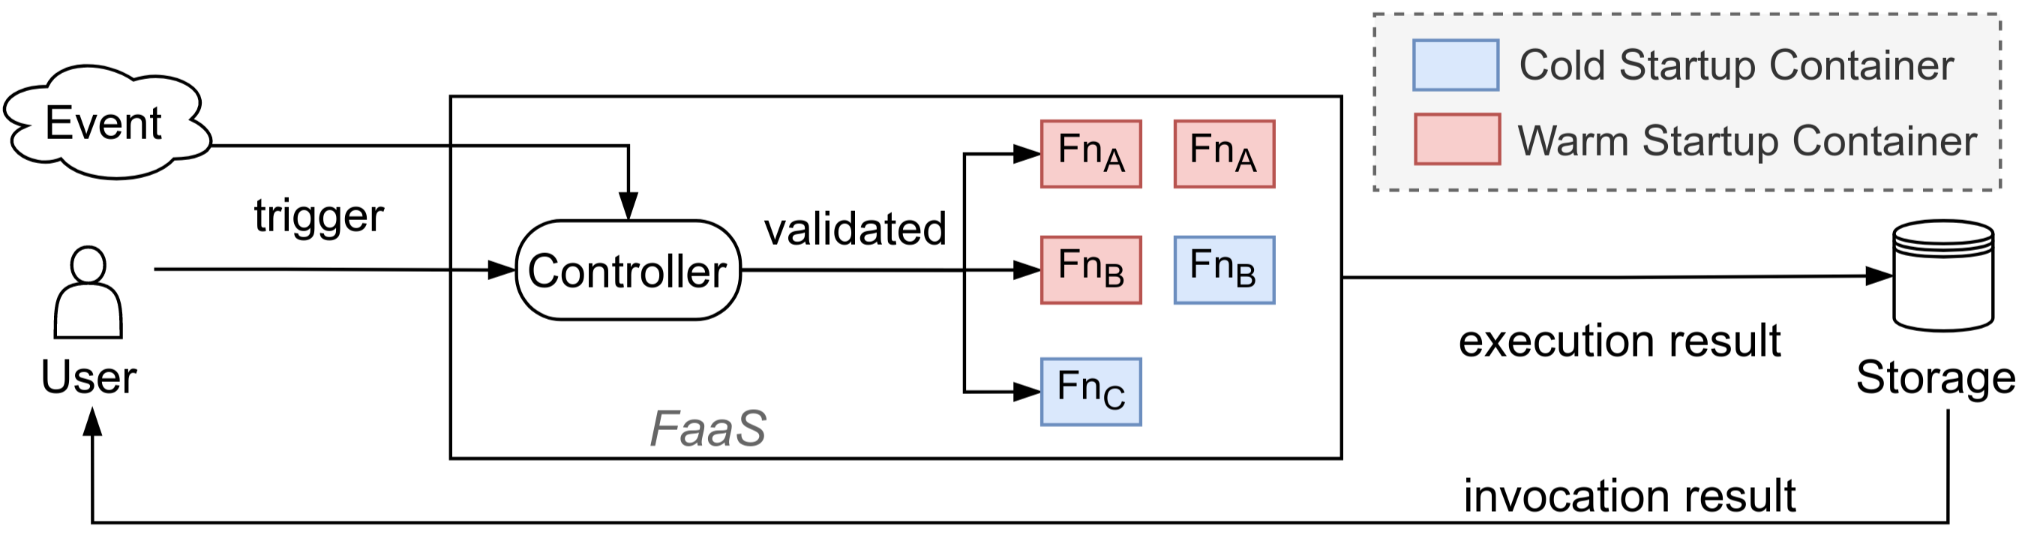
\includegraphics[width=\linewidth]{serverlessexecution.png}
	\caption{Example of an asynchronous invocation. Source: \cite{li_serverless_2022}}
	\label{fig:serverlessexecution}
\end{figure*}

\subsection{Methodology}
Serverless computing is a broad and complex field that is closely linked to various topics, such as performance, security or caching. While some publications focus on specific areas by reviewing the latest academic literature in those fields, this work adopts a broader approach in order to provide a comprehensive overview from multiple perspectives. It first analyzes surveys and articles to cover critical topics closely connected to serverless computing and, additionally, it explores innovative and notable studies addressing individual challenges, ultimately offering a holistic perspective on serverless computing.

\section{Cost-effectiveness}
\label{sec:costeffectiveness}
Serverless computing appears more expensive than traditional cloud computing at a first analysis: the per-minute execution cost of an AWS Lambda function is 7.5 times as expensive compared to an AWS t3.nano VM. As Schleier et al. observe \cite{schleier-smith_what_2021}, however, serverless providers include in the price the cost of redundancy for ensuring availability, auto-scaling, monitoring and logging, which are functionalities that are under the responsibility of developers in traditional cloud computing approaches (which this work refers to as ``serverful''), or have to be purchased as separate services.
Another benefit of serverless computing is its cost model, which follows a pay-as-you-go pricing structure. In this model, end-users are charged only for the resources they actually consume, while the cloud provider covers the costs of any idle resources, as illustrated in Figure \ref{fig:serverlesscost}.
\begin{figure*}
	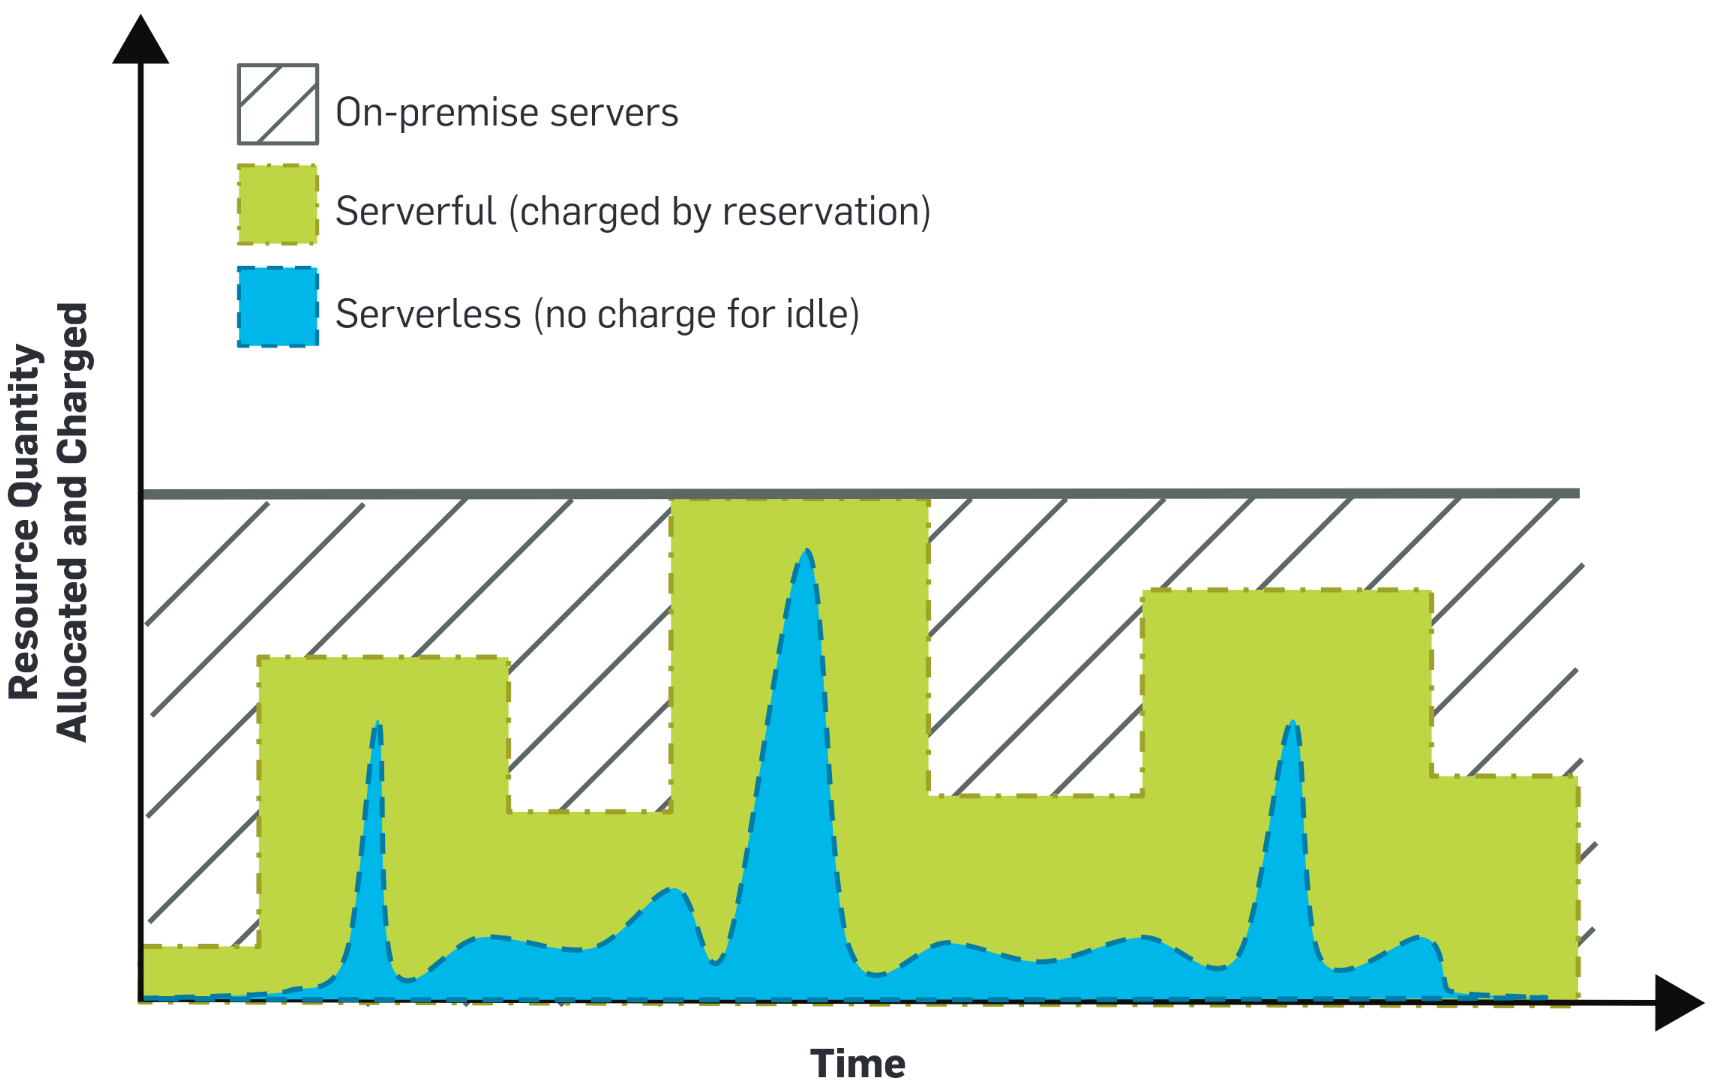
\includegraphics[width=\linewidth]{serverlesscost.png}
	\caption{Advantages of serverless computing's cost model. Source: \cite{schleier-smith_what_2021}}
	\label{fig:serverlesscost}
\end{figure*}
Even with dynamic resource allocation, serverful computing operates on a reservation model, requiring computing resources to be allocated based on the application's peak usage, which leads to a very large underutilization of resources. As Castro et al. point out \cite{schleier-smith_what_2021}, in practice, customer realize saving when moving their applications to serverless. The price reductions and the increased functionalities offered by the cloud providers could threaten their revenues, however, as noted by the Jevons Paradox \cite{alcott_jevons_2005}, lower prices and fewer customer responsibilities can stimulate demand, offsetting the price decrease and potentially boosting providers’ earnings. 

\section{Security and Privacy}
Since serverless computing is inherently event-driven and the services provided by platforms are cloud-based, authentication becomes a critical challenge: only authorized applications should be able to trigger events that start function executions on the cloud, otherwise a freeloader could take advantage of the available resources of the victims \cite{shafiei_serverless_2022}. A token-based authentication strategy could be employed, where specific tokens are included in requests, as AWS Lambda implements\footnote{\url{https://docs.aws.amazon.com/apigateway/}}; however, these tokens could be extracted and reused if the message is sent through an unsecured network. 
An effective solution would be to use SSL/TLS protocols \cite{freier_secure_2011, rescorla_transport_2018}, but it may be beyond the capabilities of low-energy IoT devices.

Using IoT devices in serverless environments is not uncommon: due to the auto-scalability property of serverless computing, it can easily handle large bursts of requests, which frequently occur when IoT systems monitor environmental conditions that can generate numerous events (consider, for example, the case of an earthquake detection network that might rapidly generate extensive data whenever seismic activity is detected). IoT applications might also be very privacy-sensitive: an example that Shafiei et al. \cite{shafiei_serverless_2022} point out is a use case in healthcare, where IoT devices transfer patient data: in this scenario, an attacker could extract sensitive information about patients only by having access to the function called and their parameters. 

Authorization is another central aspect: certain functions might be restricted to be called only by certain users or functions. To tackle this issue, AWS Lambda uses a role-based approach, where every function is associated with a particular set of permissions and users have a role that define the functions they are allowed to execute. User executions can be isolated, allowing functions to run within the caller's context, as depicted in Figure \ref{fig:authorization}. 
\begin{figure*}[!htb]
	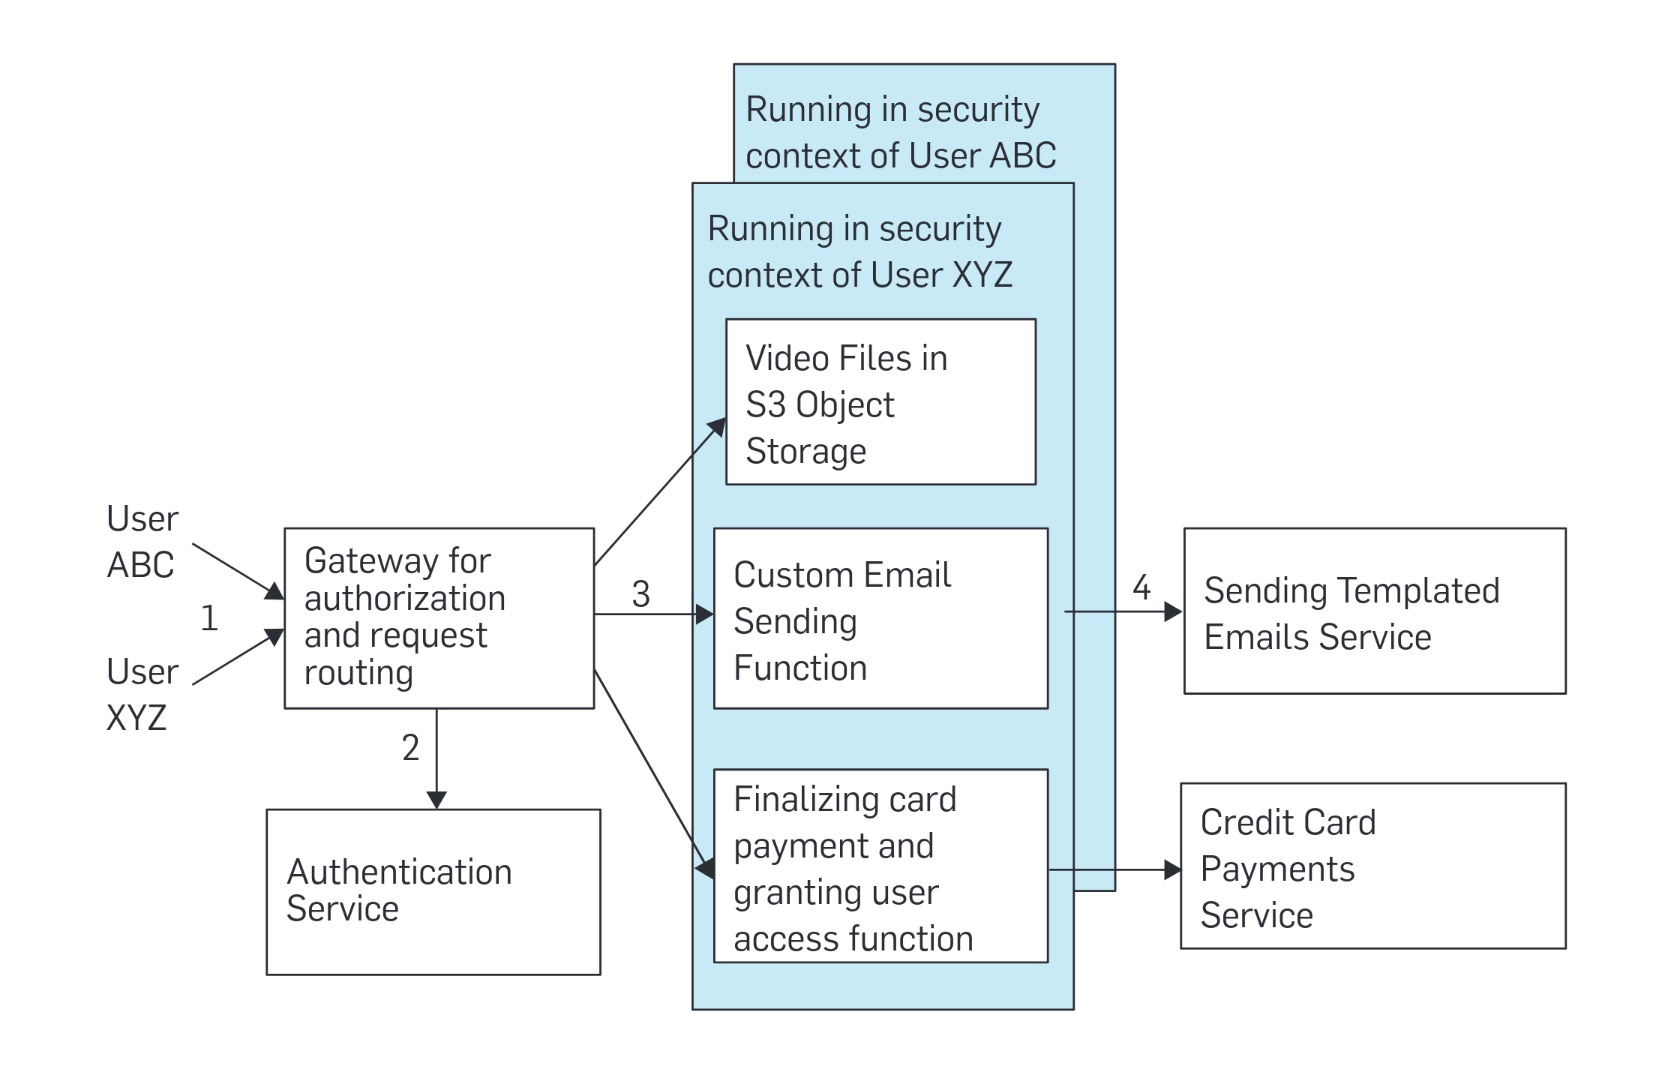
\includegraphics[width=\linewidth]{authorization.png}
	\caption{Authorization and isolated execution in serverless. Source: \cite{castro_rise_2019}}
	\label{fig:authorization}
\end{figure*}

Moreover, security concerns such as replay attacks are significant \cite{shafiei_serverless_2022}: in this type of attacks, the attacker does not know the content of a message, but is interested in the effects of its transmission; in the context of serverless, this could lead to resource exhaustion attacks in the case of multiple malicious function calls that result in a usage beyond the service-level agreement with the provider. Despite this, as Marin et al. highlight \cite{marin_serverless_2022}, the serverless paradigm is more resistant to (Distributed) Denial-of-Service attacks compared to other approaches, as it enjoys elasticity provided by its auto-scaling feature. Rather than the disruption of the service, a more common consequence of attacks is a heavy financial load on the application owner.

On the bright side, serverless can act as a security enabler under some points of view \cite{marin_serverless_2022}:
\begin{itemize}
	\item It increases difficulty in performing attacks: serverless functions are short-lived, and this imposes time limits on the adversaries to retrieve data or to reach high privileged accounts to perform further damage.
	\item It relieves developers of some security concerns: security becomes a shared concern between the developers and the providers. Providers take care of many security tasks, especially related to the infrastructure; however, developers still need to the heavily involved in security matters, securing their workflows by preventing functions' vulnerabilities, limiting execution privileges and securing the data on the cloud. 
\end{itemize}

\section{Data Caching}
\label{sec:caching}
\begin{figure*}[!hbt]
	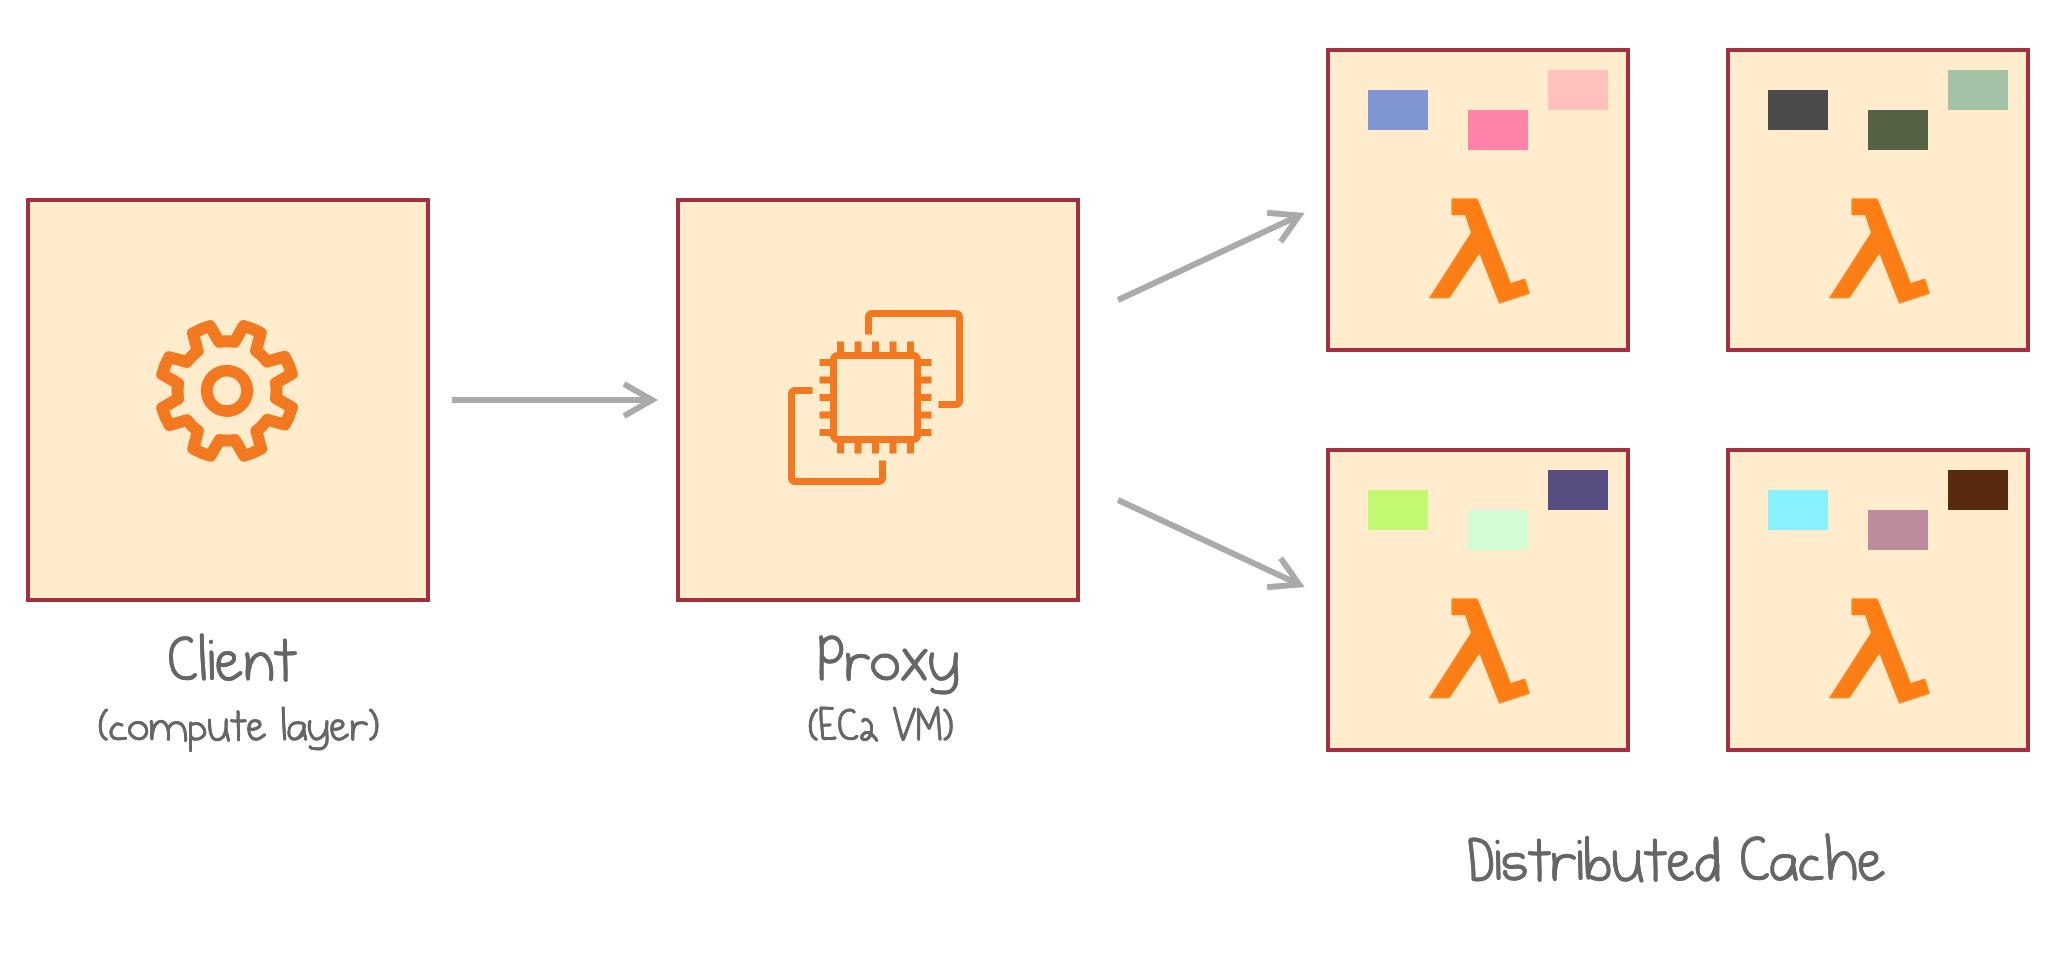
\includegraphics[width=\linewidth]{infinicache.png}
	\caption{InfiniCache workflow. Source: \href{https://mikhail.io/2020/03/infinicache-distributed-cache-on-aws-lambda/}{www.mikhail.io}}
	\label{fig:infinicache}
\end{figure*}
Applications across various domains frequently rely on querying databases to retrieve and manipulate data essential for their functionalities, which in the case of serverless platforms are cloud databases. Querying cloud databases may result in bottlenecks due to the latencies of persistent storage. Serverful systems use multiple level of caches, but this approach can be challenging to implement in serverless environments, given the stateless nature of the functions.
Since a lack of caching makes the serverless services infeasible in real-world scenarios, there were various attempts to implement caching, mainly in-memory and distributed on multiple nodes. Amazon developed ElastiCache\footnote{\url{https://aws.amazon.com/elasticache/}}, an in-memory cache and data store, but it is at least 700 times more expensive compared to Amazon S3 (Amazon's cloud storage service\footnote{\url{https://aws.amazon.com/s3/}}) \cite{shafiei_serverless_2022}, therefore, open source alternatives such as InfiniCache \cite{wang_infinicache_nodate} were also implemented. 
The implementation of a distributed cache is not straightforward\footnote{An in-depth explanation of the problem can be found at \url{https://mikhail.io/2020/03/infinicache-distributed-cache-on-aws-lambda/}}: a first idea that might come to mind is caching data between requests in an in-memory hashmap; however, the size of functions is limited to some gigabytes by serverless providers, and every instance of the same function would need to keep in the memory potentially the same data (for example, in the case of parallel requests).
Another option would be to implement a simple distributed caching system by moving the cache in multiple functions (units of execution) that contains a portion of the data, a big upside of this approach would be the caching pay model: cost is charged only when cache functionalities are used (i.e. function instances are running), while cluster-based services charge for memory capacity whether cached objects are accessed or not.
However, serverless functions are not designed for stateful use cases: they have limited resources (both CPU and memory-wise) and can run for some minutes at most. Moreover, providers such as AWS Lambda reserve the right to terminate idle functions at any time.
InfiniCache tackles these problems with a component (referred in \cite{wang_infinicache_nodate} as \textit{Proxy}) that manages multiple functions that hold slices of data. Clients communicates with the proxy, which orchestrates the caching transparently from them, as depicted in Figure \ref{fig:infinicache}.
Since InfiniCache is implemented on AWS Lambda, where the provider can claim idle instances at any time, it implements a backup mechanism for cache functions, creating redundancy with multiple functions containing the same data. In this way, if the proxy has to retrieve data in the cache, but the primary instance containing the requested data was shut down, it can reroute the request to its backup.
On AWS Lambda the functions cannot receive TCP or UDP connections; therefore, to allow communication with the proxy, the proxy's IP and port are passed as parameters during the function invocation and the function itself starts a TCP connection towards the Proxy during initialization, as shown in Figure \ref{fig:lambdainvocation}. 
\begin{figure}[!hbt]
	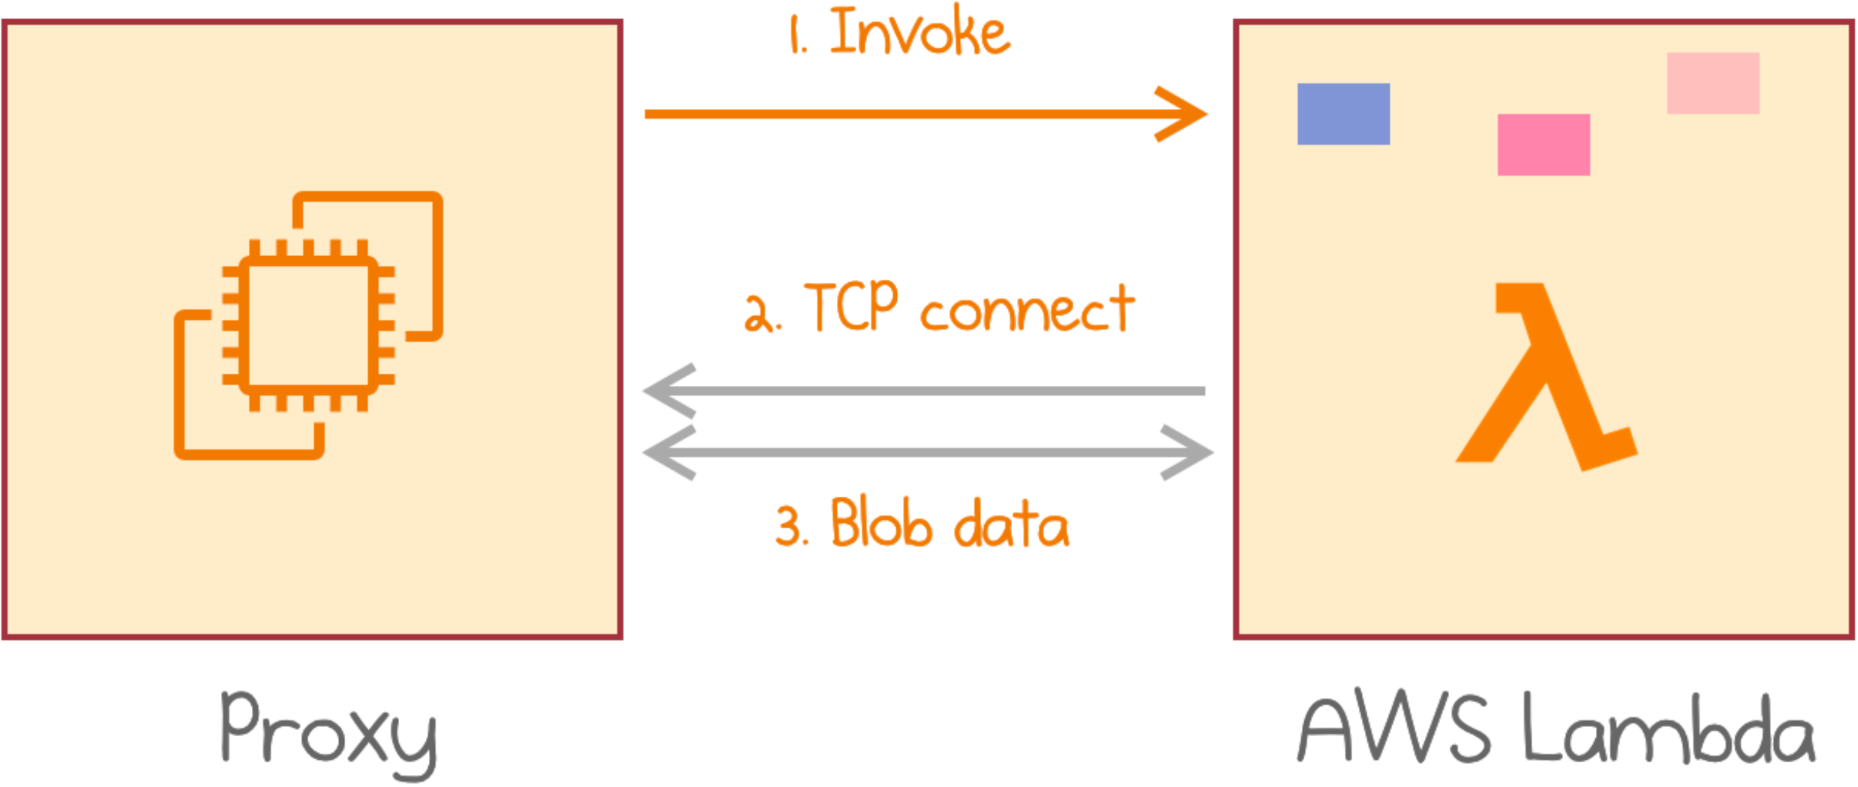
\includegraphics[width=\linewidth]{lambdainvocation.png}
	\caption{Invocation of a function and connection to the proxy. Source: \href{https://mikhail.io/2020/03/infinicache-distributed-cache-on-aws-lambda/}{www.mikhail.io}}
	\label{fig:lambdainvocation}
\end{figure}
\section{Performance}
\label{sec:performance}

\begin{figure}[!hbt]
	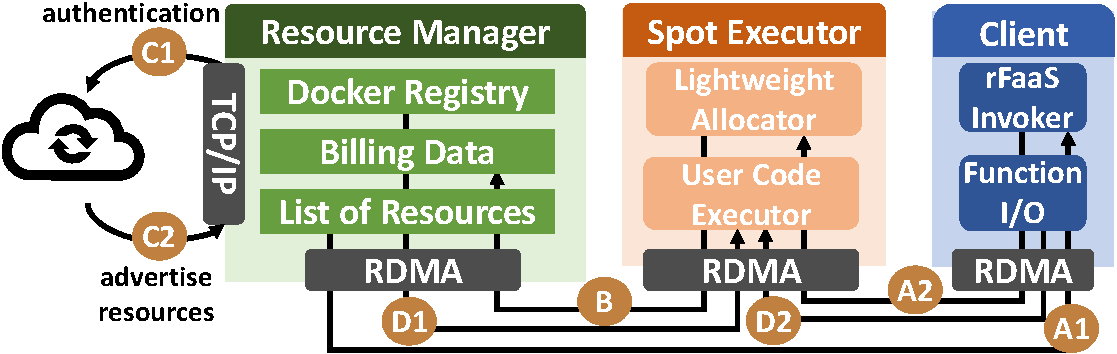
\includegraphics[width=\linewidth]{rfaas.pdf}
	\caption{Architecture of rFaaS: clients acquire leases (\circledColorSmall{A}{brown}) and invoke functions (\circledColorSmall{D}{brown}), spot executors manage execution environments, resource managers interact with data center resources (\circledColorSmall{C}{brown}) and manage billing (\circledColorSmall{B}{brown}). Source: \cite{copik_rfaas_2023}}
	\label{fig:rfaas}
\end{figure}

While modern cloud paradigms can bring elasticity to allocate idle resources and even reduce computational costs, as shown in Section \ref{sec:costeffectiveness}, its performance cannot match cluster allocations and coarse-grained cloud executions. Serverless poses some limitations to High-Performance Computing applications, since many platforms make use of centralized scheduling with a high number of parties involved in functions executions that increase execution latencies. Moreover, inefficient network transport protocols are used, limiting the use of serverless for latency-sensitive applications. To limit these issues and make serverless a feasible option for the aforementioned applications, \textit{rFaaS}, a Remote Direct Access Memory (RDMA) accelerated FaaS platform, aims to reduce execution latencies by limiting the overhead on the fastest available network.

rFaaS introduces various components, as depicted in Figure \ref{fig:rfaas}. \textbf{Spot executors} are entities that provide hardware and software resources to clients, to support the execution of serverless functions; each spot executor is assigned a part of the available resources.
A spot executor includes:
\begin{itemize}
	\item \textbf{User code executors}, executor processes responsible for the execution of client code
	\item A \textbf{lightweight allocator}, which is responsible for connecting new clients (\circledColorSmall{A2}{brown}), managing code executors and the processes that are being executed and removing processes that are idle or that are exceeding specific time limits
\end{itemize}
When a client wants to execute code it connects to a spot executor which initializes an isolated execution context with a user code executor, that can be implemented as a bare-metal process or a Docker container (\circledColorSmall{D1}{brown}). The client can then leverage the RDMA capabilities of the service to write functions headers and payloads directly to the code executor's memory (\circledColorSmall{D2}{brown}). Spot executors are managed by entities called \textbf{resource managers}: each one is assigned a group of spot executors and interacts with data center resources (\circledColorSmall{C}{brown}), assigning them to spot executors when they become available. Resource managers also handle billing data for the clients (\circledColorSmall{B}{brown}). An important concept introduced by rFaaS to speedup consecutive invocations is \textbf{leasing}: clients acquire leases on executor processes, and leverage them to perform consecutive executions on warmed up containers. Leases allow to avoid the initialization costs of reliable RDMA connections and limit the interaction between clients and resource managers: the latter is involved only once to acquire a lease (\circledColorSmall{A1}{brown}), and not every time a function is invoked. The separation of concerns between resource managers and spot executors allows to reduce the critical path of invocations by removing a centralized gateway, ultimately reducing the number of parties involved in transmitting functions data. 

To reduce the startup delays, alongside warm and cold executions, rFaaS introduces the concept of hot invocations, a sandbox state where, after a request is completed, the threads continue to active poll for invocation requests. Busy polling decreases the invocation latency since threads do not enter blocked states waiting for RDMA events. This operation comes at the cost of occupying the CPU, and so it should be considered as active computation time; the executors can switch back to normal warm mode after a configurable amount of time to free the CPU. 

The use of hot containers decreases the overall overhead to about 350 nanoseconds on top of the fastest available network transmission. While this implementation of a RMDA-accelerated serverless platform requires specific hardware and lacks some features offered by cloud providers, such as shared storage, it is a great attempt to adapt serverless computing to scenarios with strict latency constraints.


\section{Scheduling}
Section \ref{sec:performance} described an alternative architecture that can optimize scheduling, but most providers use a different architecture where functions scheduling is transparent from the end users. However, these providers can still optimize scheduling based on many parameters. Shafiei et al. \cite{shafiei_serverless_2022} provide an in-depth analysis of the various scheduling policies available. 

\subsection{Resource Consumption Patterns}
There is various information that is useful to know for the provider to ensure proper scheduling. Understanding data consumption patterns of tasks that are executed is crucial; for instance, if multiple CPU-intensive functions run on the same physical machine, it may lead to resource contention. Similarly, tasks that transfer large amounts of data over the network could introduce communication delays if they are co-located on the same machine. Therefore, a resource-aware scheduling can take these applications needs into account to limit the concurrent high demand on shared hardware resources.

\subsection{Reducing Startup Overhead}
Delays in serverless applications have multiple causes, including cold container startups, remote database queries and dependency installations, as explained in Sections \ref{sec:caching} and \ref{sec:performance}. Providers can aim to mitigate these issues by incorporating predictive and speculative scheduling. In fact, serverless applications rarely involve only one function invocation, but they are mostly made by chain of invocations, where multiple functions are called concurrently or a function invocates other functions. Providers could prepare warm containers based on known or anticipated invocation patterns, reducing startup overhead. Functions can often install dependencies as well, and batching together executions that require to download the same dependencies can further reduce overheads.

\subsection{Data Locality}
While functions are stateless, it is not uncommon to depend on external data sources to perform the computations; therefore, scheduling strategies increasingly prioritize data locality. By placing functions closer to the data they process, providers can significantly reduce data transfer latencies, improving overall applications' performance.

\section{Statistics on serverless usage}
Despite the leading serverless platform (AWS Lambda) was launched in 2015, serverless is still trending and growing. Datadog stated in its last report\footnote{\href{https://www.datadoghq.com/state-of-serverless/}{https://www.datadoghq.com/state-of-serverless/}} that AWS Lambda grew by 3\% from 2022 to 2023, while Azure and Google Cloud grew by 6\% and 7\% respectively. Python and Node.js are the leading languages used in serverless environments, and for good reasons: the average startup time of functions written in Java (which is the third leading language) is two times longer compared to Python or Node.js. The reason is that startup time is influenced by the memory allocated to a function, and more than 25\% of all Java functions allocate more than 1024 MB per function, compared to only about 10\% of functions written in Python and Node.js.

\subsection{Functions Marketplaces}
Functions marketplaces offer pre-built serverless functions to be easily deployed; the most notable example is the AWS Serverless Application Repository\footnote{https://serverlessrepo.aws.amazon.com/applications}, that counts more than 1100 functions. As Shafiei et al. \cite{shafiei_serverless_2022} point out, the competition on these platforms could result in an increase of functions quality, ultimately in favor of the customers. 

Spillner \cite{spillner_quantitative_2019} provides a quantitative analysis of the functions in the AWS Serverless Application Repository. Although the report dates back to 2019, when the repository had roughly half of the functions it has today, the conclusion are partially analogous to the ones in the Datadog report cited above, particularly about the dominance of Python and Node.js as the leading programming languages for serverless.


\section{Conclusion}
Serverless computing represents a transformative shift in the cloud computing paradigm, and porting applications to serverless environments would offer benefits such as cost-efficiency, automated scalability, and simplified infrastructure management. Its pay-as-you-go model has unlocked new possibilities for businesses and developers, allowing them to focus on innovation rather than operational complexities. However, this is not without challenges, since the stateless nature of the paradigm and its latencies compared to typical serverful implementations can limit its expansion, and need to be addressed. 

Through this work, an overview on the topic under many points of view was provided, highlighting not only the paradigm's potentialities but also the challenges serveless computing is facing; and previous innovative efforts that aim to limit or solve some limitations were analyzed. Addressing these limitations is crucial for serverless computing to mature into a more robust, adaptable, and widely applicable technology for the future of cloud services.

% \begin{equation}
% 	\cos^3 \theta =\frac{1}{4}\cos\theta+\frac{3}{4}\cos 3\theta
% 	\label{eq:example}
% \end{equation}

% Automatically referencing an equation number using its label: Equation \ref{eq:example}.

% In hac habitasse platea dictumst. Curabitur mattis elit sit amet justo luctus vestibulum. In hac habitasse platea dictumst. Pellentesque lobortis justo enim, a condimentum massa tempor eu. Ut quis nulla a quam pretium eleifend nec eu nisl. Nam cursus porttitor eros, sed luctus ligula convallis quis. Nam convallis, ligula in auctor euismod, ligula mauris fringilla tellus, et egestas mauris odio eget diam. Praesent sodales in ipsum eu dictum. Aenean vel enim ipsum. Fusce ut felis at eros sagittis bibendum mollis lobortis libero.

% Maecenas consectetur metus at tellus finibus condimentum. Proin arcu lectus, ultrices non tincidunt et, tincidunt ut quam. Integer luctus posuere est, non maximus ante dignissim quis. Nunc a cursus erat. Curabitur suscipit nibh in tincidunt sagittis. Nam malesuada vestibulum quam id gravida. Proin ut dapibus velit. Vestibulum eget quam quis ipsum semper convallis. Duis consectetur nibh ac diam dignissim, id condimentum enim dictum. Nam aliquet ligula eu magna pellentesque, nec sagittis leo lobortis. Aenean tincidunt dignissim egestas.

% %------------------------------------------------

% \section{Methodologies}

% \subsection{Sample Sites \& Processing}

% This line shows how to use a footnote to further explain or cite text\footnote{Example footnote text.}.

% This is a bullet point list:

% \begin{itemize}
% 	\item Arcu eros accumsan lorem, at posuere mi diam sit amet tortor
% 	\item Fusce fermentum, mi sit amet euismod rutrum
% 	\item Sem lorem molestie diam, iaculis aliquet sapien tortor non nisi
% 	\item Pellentesque bibendum pretium aliquet
% \end{itemize}

% Mauris interdum porttitor fringilla. Proin tincidunt sodales leo at ornare. Donec tempus magna non mauris gravida luctus. Cras vitae arcu vitae mauris eleifend scelerisque. Nam sem sapien, vulputate nec felis eu, blandit convallis risus. Pellentesque sollicitudin venenatis tincidunt. In et ipsum libero. Nullam tempor ligula a massa convallis pellentesque.

% This is a numbered list:

% \begin{enumerate}
% 	\item Donec dolor arcu, rutrum id molestie in, viverra sed diam
% 	\item Curabitur feugiat
% 	\item Turpis sed auctor facilisis
% \end{enumerate}

% \subsection{Species Identification}

% Proin lobortis efficitur dictum. Pellentesque vitae pharetra eros, quis dignissim magna. Sed tellus leo, semper non vestibulum vel, tincidunt eu mi. Aenean pretium ut velit sed facilisis. Ut placerat urna facilisis dolor suscipit vehicula. Ut ut auctor nunc. Nulla non massa eros. Proin rhoncus arcu odio, eu lobortis metus sollicitudin eu. Duis maximus ex dui, id bibendum diam dignissim id. Aliquam quis lorem lorem. Phasellus sagittis aliquet dolor, vulputate cursus dolor convallis vel. Suspendisse eu tellus feugiat, bibendum lectus quis, fermentum nunc. Nunc euismod condimentum magna nec bibendum. Curabitur elementum nibh eu sem cursus, eu aliquam leo rutrum. Sed bibendum augue sit amet pharetra ullamcorper. Aenean congue sit amet tortor vitae feugiat.

% Mauris interdum porttitor fringilla. Proin tincidunt sodales leo at ornare. Donec tempus magna non mauris gravida luctus. Cras vitae arcu vitae mauris eleifend scelerisque. Nam sem sapien, vulputate nec felis eu, blandit convallis risus. Pellentesque sollicitudin venenatis tincidunt. In et ipsum libero. Nullam tempor ligula a massa convallis pellentesque.

% \subsection{Data Analysis}

% Vestibulum sodales orci a nisi interdum tristique. In dictum vehicula dui, eget bibendum purus elementum eu. Pellentesque lobortis mattis mauris, non feugiat dolor vulputate a. Cras porttitor dapibus lacus at pulvinar. Praesent eu nunc et libero porttitor malesuada tempus quis massa. Aenean cursus ipsum a velit ultricies sagittis. Sed non leo ullamcorper, suscipit massa ut, pulvinar erat. Aliquam erat volutpat. Nulla non lacus vitae mi placerat tincidunt et ac diam. Aliquam tincidunt augue sem, ut vestibulum est volutpat eget. Suspendisse potenti. Integer condimentum, risus nec maximus elementum, lacus purus porta arcu, at ultrices diam nisl eget urna. Curabitur sollicitudin diam quis sollicitudin varius. Ut porta erat ornare laoreet euismod. In tincidunt purus dui, nec egestas dui convallis non. In vestibulum ipsum in dictum scelerisque.

% Mauris interdum porttitor fringilla. Proin tincidunt sodales leo at ornare. Donec tempus magna non mauris gravida luctus. Cras vitae arcu vitae mauris eleifend scelerisque. Nam sem sapien, vulputate nec felis eu, blandit convallis risus. Pellentesque sollicitudin venenatis tincidunt. In et ipsum libero. Nullam tempor ligula a massa convallis pellentesque. Mauris interdum porttitor fringilla. Proin tincidunt sodales leo at ornare. Donec tempus magna non mauris gravida luctus. Cras vitae arcu vitae mauris eleifend scelerisque. Nam sem sapien, vulputate nec felis eu, blandit convallis risus. Pellentesque sollicitudin venenatis tincidunt. In et ipsum libero. Nullam tempor ligula a massa convallis pellentesque.

% %------------------------------------------------

% \section{Results}

% \begin{table} % Single column table
% 	\caption{Example single column table.}
% 	\centering
% 	\begin{tabular}{l l r}
% 		\toprule
% 		\multicolumn{2}{c}{Location} \\
% 		\cmidrule(r){1-2}
% 		East Distance & West Distance & Count \\
% 		\midrule
% 		100km & 200km & 422 \\
% 		350km & 1000km & 1833 \\
% 		600km & 1200km & 890 \\
% 		\bottomrule
% 	\end{tabular}
% 	\label{tab:distcounts}
% \end{table}

% Referencing a table using its label: Table \ref{tab:distcounts}.

% \begin{table*} % Full width table (notice the starred environment)
% 	\caption{Example two column table with fixed-width columns.}
% 	\centering % Horizontally center the table
% 	\begin{tabular}{L{0.2\linewidth} L{0.2\linewidth} R{0.15\linewidth}} % Manually specify column alignments with L{}, R{} or C{} and widths as a fixed amount, usually as a proportion of \linewidth
% 		\toprule
% 		\multicolumn{2}{c}{Location} \\
% 		\cmidrule(r){1-2}
% 		East Distance & West Distance & Count \\
% 		\midrule
% 		100km & 200km & 422 \\
% 		350km & 1000km & 1833 \\
% 		600km & 1200km & 890 \\
% 		\bottomrule
% 	\end{tabular}
% \end{table*}

% Aenean feugiat pellentesque venenatis. Sed faucibus tristique tortor vel ultrices. Donec consequat tellus sapien. Nam bibendum urna mauris, eget sagittis justo gravida vel. Mauris nisi lacus, malesuada sit amet neque ut, venenatis tempor orci. Curabitur feugiat sagittis molestie. Duis euismod arcu vitae quam scelerisque facilisis. Praesent volutpat eleifend tortor, in malesuada dui egestas id. Donec finibus ac risus sed pellentesque. Donec malesuada non magna nec feugiat. Mauris eget nibh nec orci congue porttitor vitae eu erat. Sed commodo ipsum ipsum, in elementum neque gravida euismod. Cras mi lacus, pulvinar ut sapien ut, rutrum sagittis dui. Donec non est a metus varius finibus. Pellentesque rutrum pellentesque ligula, vitae accumsan nulla hendrerit ut.

% \begin{figure} % Single column figure
% 	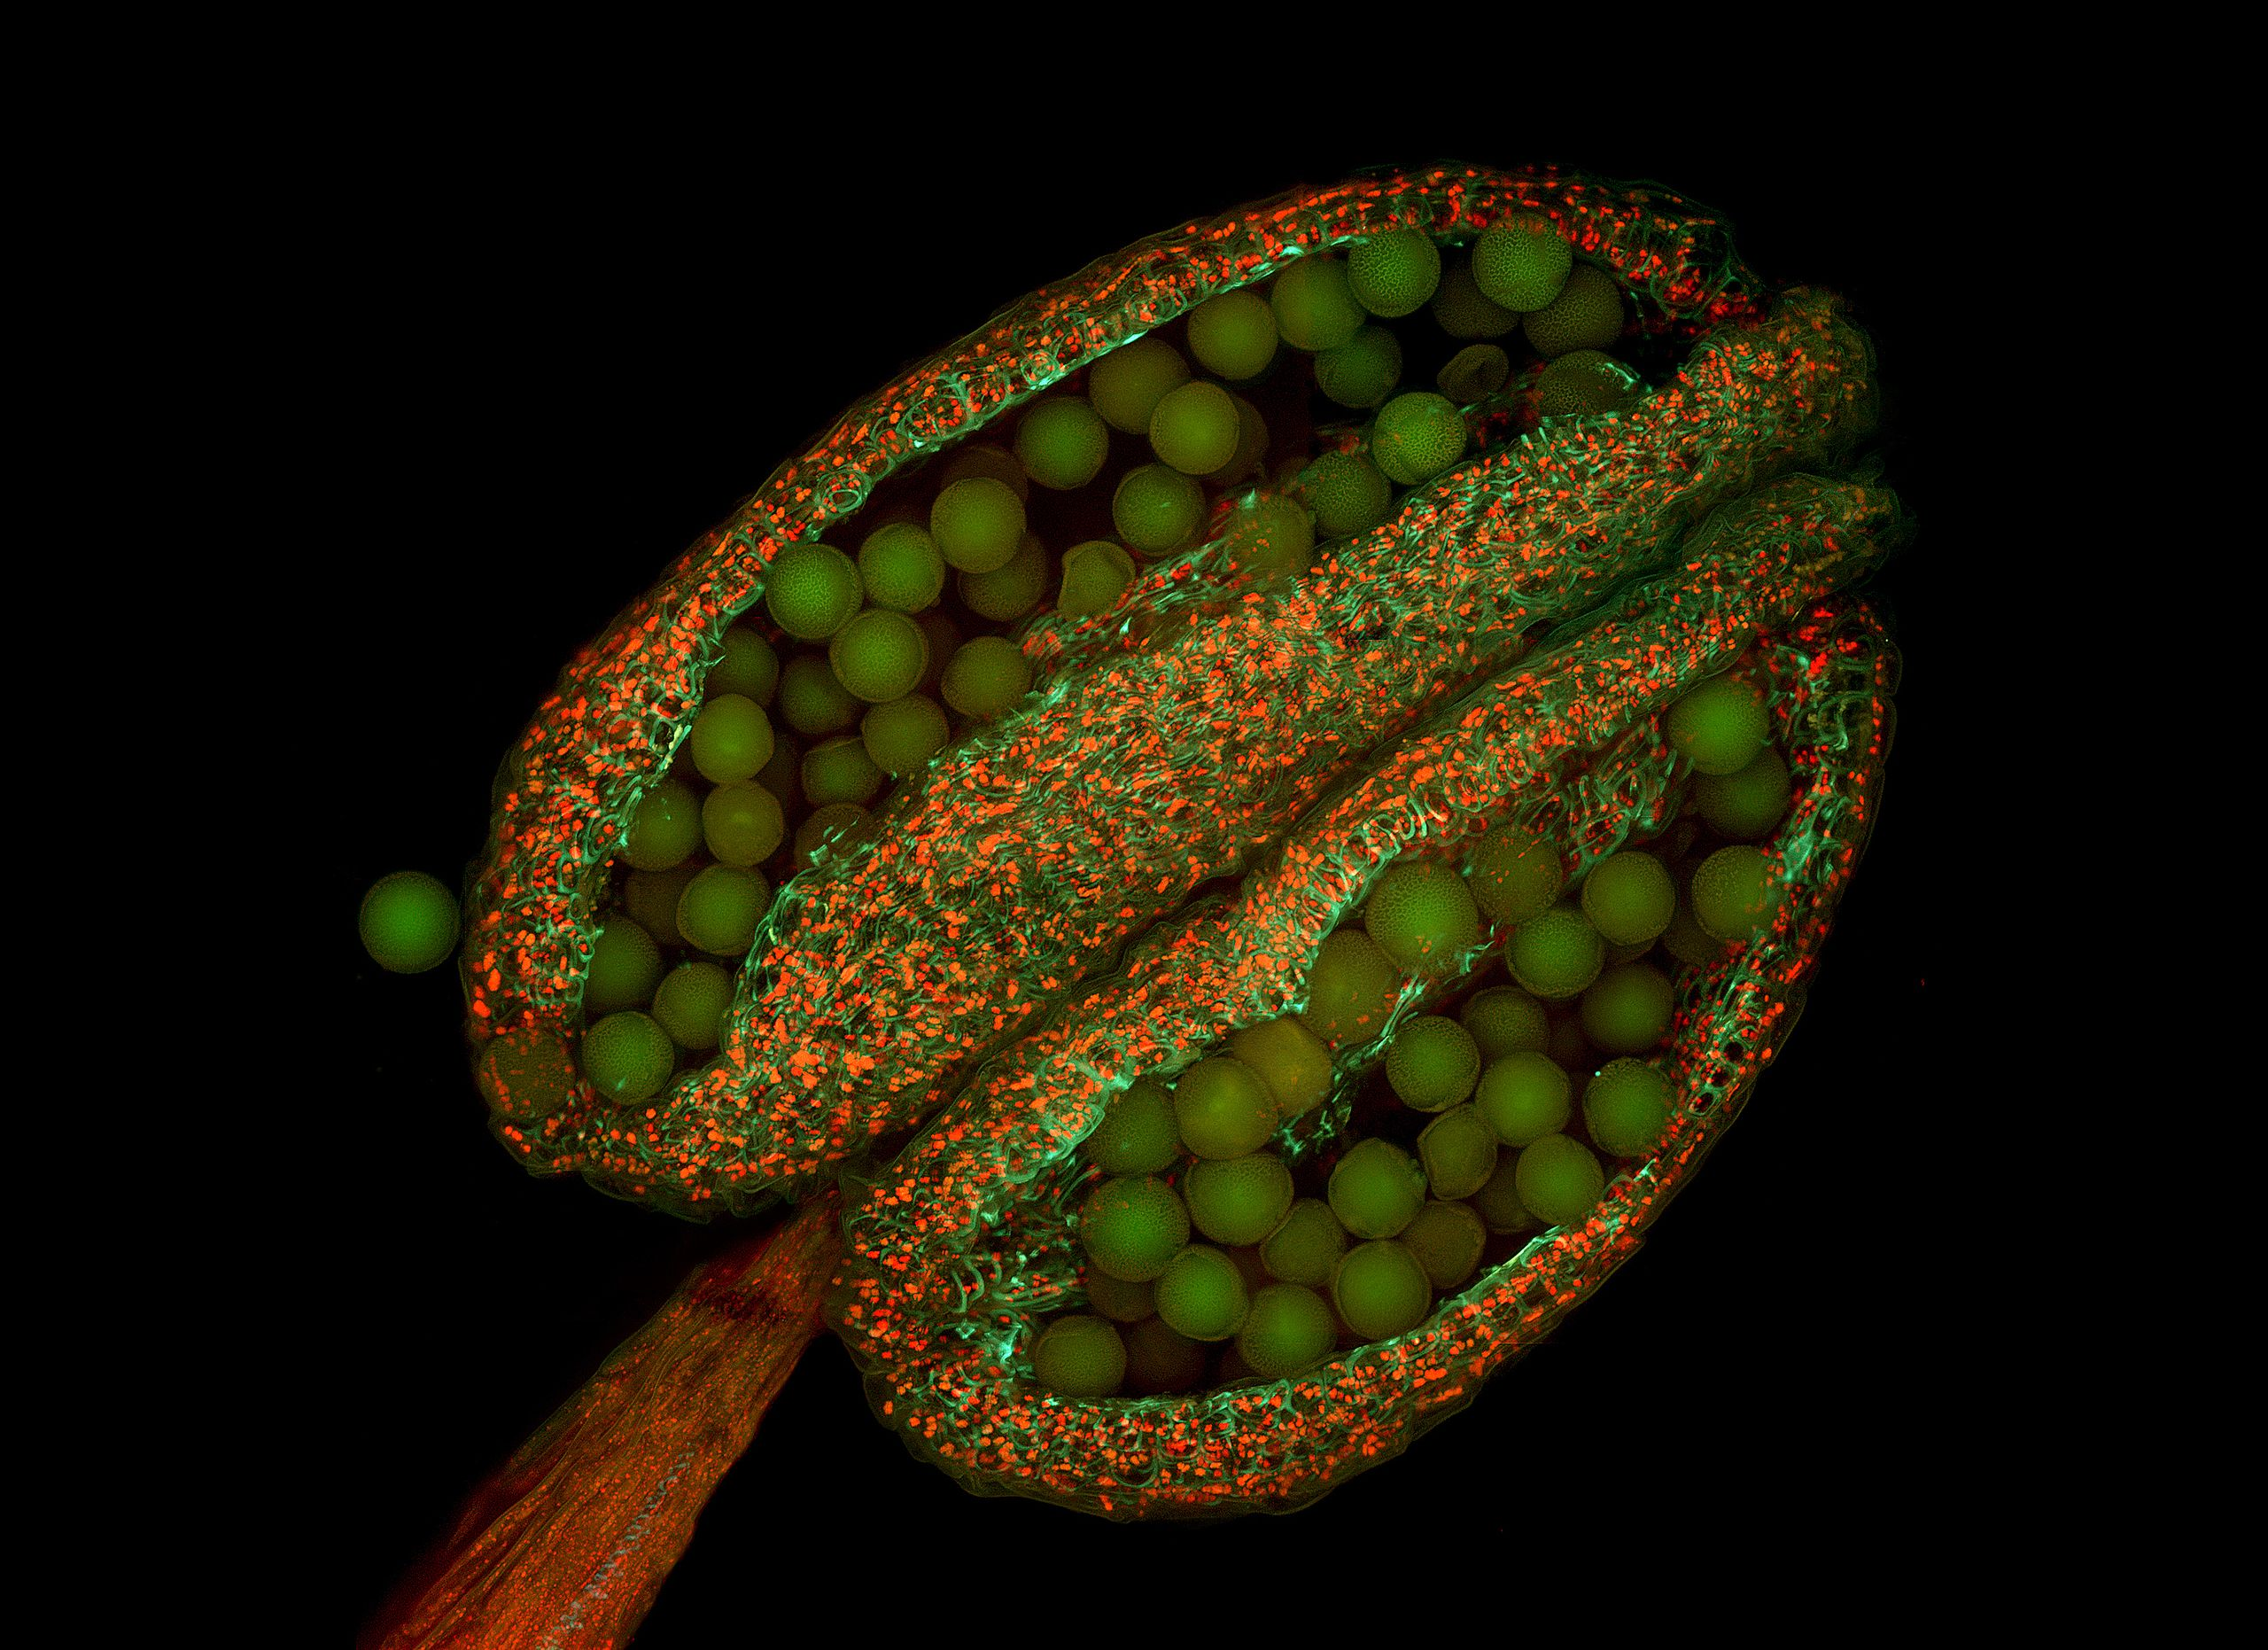
\includegraphics[width=\linewidth]{Tolmukapea.jpg}
% 	\caption{Anther of thale cress (Arabidopsis thaliana), fluorescence micrograph. Source: Heiti Paves, \href{https://commons.wikimedia.org/wiki/File:Tolmukapea.jpg}{https://commons.wiki-\\media.org/wiki/File:Tolmukapea.jpg}.}
% 	\label{fig:tcanther}
% \end{figure}

% Referencing a figure using its label: Figure \ref{fig:tcanther}.

% Aenean porttitor eros non pharetra congue. Proin in odio in dolor luctus auctor ac et mi. Etiam euismod mi sed lectus fringilla pretium. Phasellus tristique maximus lectus et sodales. Mauris feugiat ligula quis semper luctus. Nam sit amet felis sed leo fermentum aliquet. Mauris arcu dui, posuere id sem eget, cursus pulvinar mi. Donec nec lacus non lectus fermentum scelerisque et at nibh. Sed tristique, metus ac vestibulum porta, tortor lectus placerat lorem, et convallis tellus dolor eget ante. Pellentesque dui ligula, hendrerit a purus et, volutpat tempor lectus. Mauris nec purus nec mauris rhoncus pellentesque. Quisque quis diam sed est lacinia congue. Donec magna est, hendrerit sed metus vel, accumsan rutrum nibh.

% \begin{figure*} % Two column figure (notice the starred environment)
% 	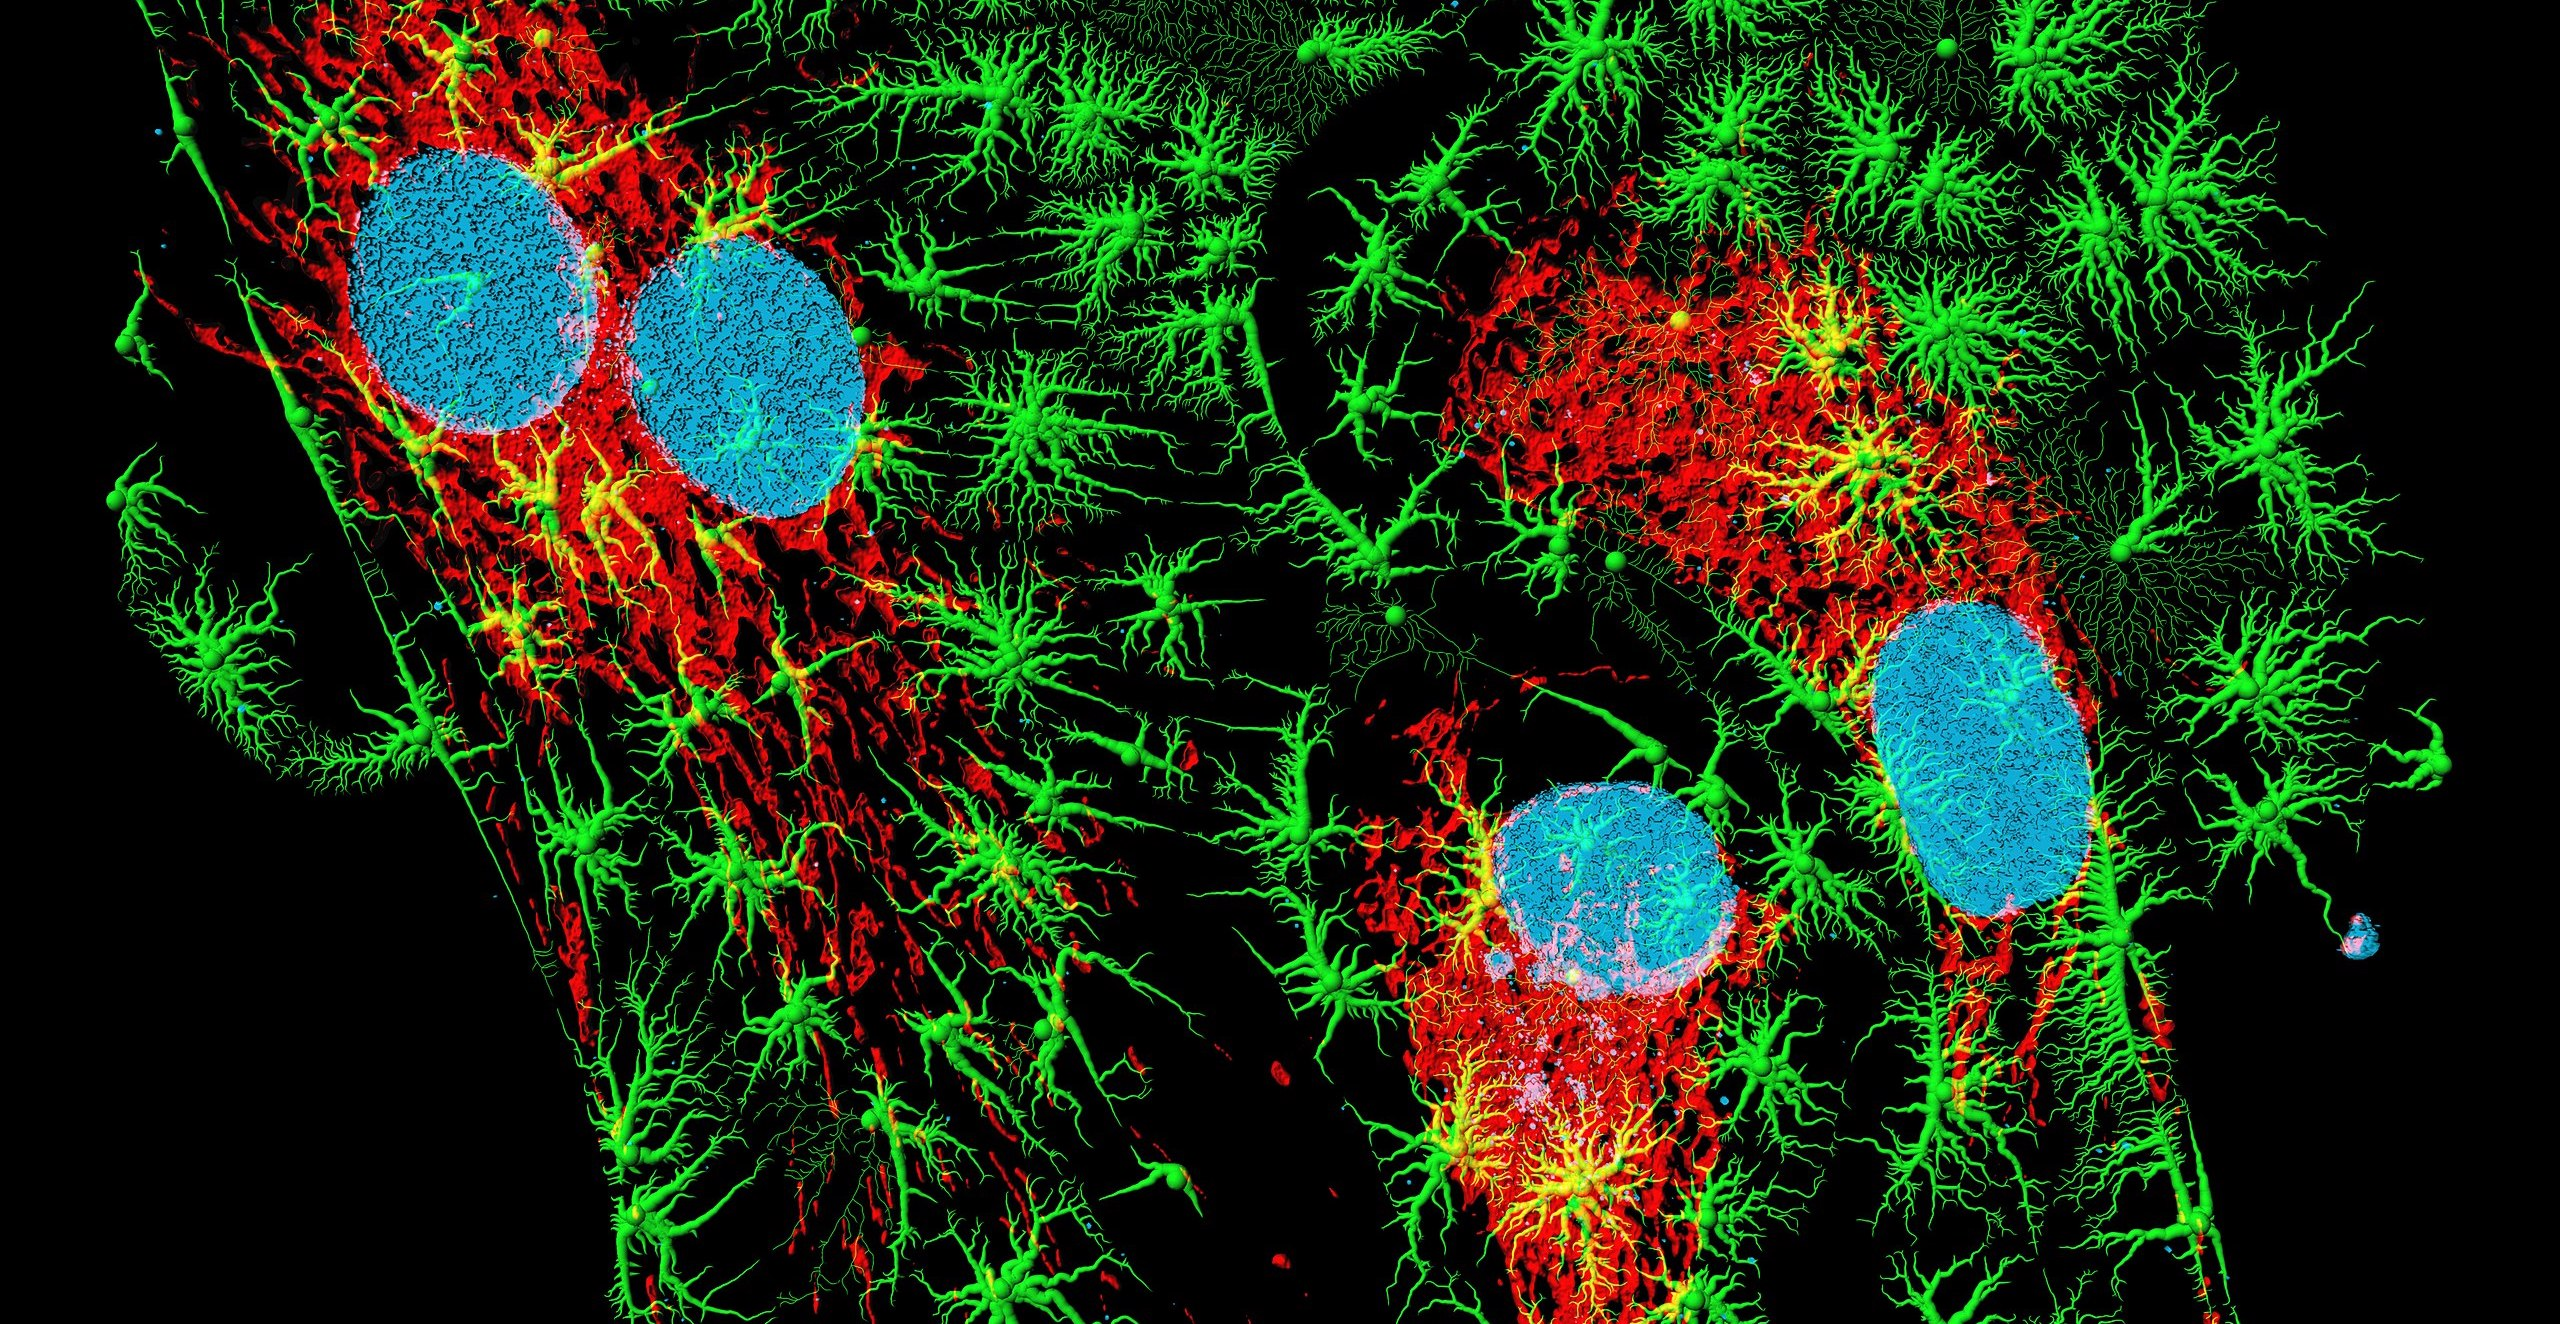
\includegraphics[width=\linewidth]{Fibroblastid.jpg}
% 	\caption{Bovine pulmonary artery endothelial cells in culture. Blue: nuclei; red: mitochondria; green: microfilaments. Computer generated image from a 3D model based on a confocal laser scanning microscopy using fluorescent marker dyes. Source: Heiti Paves, \href{https://commons.wikimedia.org/wiki/File:Fibroblastid.jpg}{https://commons.wikimedia.org/wiki/File:Fibroblastid.jpg}.}
% 	\label{fig:bpartery}
% \end{figure*}

% Orci varius natoque penatibus et magnis dis parturient montes, nascetur ridiculus mus. Etiam cursus lectus purus, tempus iaculis quam dictum tristique. Nam interdum sapien nec tempor mattis. Quisque id sapien nisi. Mauris vehicula ornare eros vel efficitur. Nulla consectetur, turpis quis fringilla tincidunt, mi neque iaculis lectus, vel commodo elit odio non ex. Duis facilisis, purus ac viverra iaculis, turpis lectus ultrices ante, ac vestibulum ligula magna in libero. Etiam tristique maximus lacinia. Vestibulum hendrerit, lacus malesuada laoreet blandit, sapien velit sollicitudin nunc, eu porttitor urna ligula at lorem. Aliquam faucibus eros in fermentum venenatis. Fusce consectetur congue pellentesque. Suspendisse at nisi sit amet est porttitor cursus. Cras placerat faucibus nunc, a laoreet justo dignissim sit amet.

% \subsection{International Support}

% \noindent àáâäãåèéêëìíîïòóôöõøùúûüÿýñçčšž

% \noindent ÀÁÂÄÃÅÈÉÊËÌÍÎÏÒÓÔÖÕØÙÚÛÜŸÝÑ

% \noindent ßÇŒÆČŠŽ

% \subsection{Links}

% This is a clickable URL link: \href{https://www.latextemplates.com}{LaTeX Templates}. This is a clickable email link: \href{mailto:vel@latextemplates.com}{vel@latextemplates.com}. This is a clickable monospaced URL link: \url{https://www.LaTeXTemplates.com}.

% %------------------------------------------------

% \section{Discussion}

% This statement requires citation \autocite{Smith:2023qr}. This statement requires multiple citations \autocite{Smith:2023qr, Smith:2024jd}. This statement contains an in-text citation, for directly referring to a citation like so: \textcite{Smith:2024jd}.

% \subsection{Subsection One}

% Suspendisse potenti. Vivamus suscipit dapibus metus. Proin auctor iaculis ex, id fermentum lectus dapibus tristique. Nullam maximus eros eget leo pretium dapibus. Nunc in auctor erat, id interdum risus. Suspendisse aliquet vehicula accumsan. In vestibulum efficitur dictum. Sed ultrices, libero nec fringilla feugiat, elit massa auctor ligula, vehicula tempor ligula felis in lectus. Suspendisse sem dui, pharetra ut sodales eu, suscipit sit amet felis. Donec pretium viverra ante, ac pulvinar eros. Suspendisse gravida consectetur urna. Pellentesque vitae leo porta, imperdiet eros eget, posuere sem. Praesent eget leo efficitur odio bibendum condimentum sit amet vel ex. Nunc maximus quam orci, quis pulvinar nibh eleifend ac. Quisque consequat lacus magna, eu posuere tellus iaculis ac. Sed vitae tortor tincidunt ante sagittis iaculis.

% \subsection{Subsection Two}

% Nullam mollis tellus lorem, sed congue ipsum euismod a. Donec pulvinar neque sed ligula ornare sodales. Nulla sagittis vel lectus nec laoreet. Nulla volutpat malesuada turpis at ultricies. Ut luctus velit odio, sagittis volutpat erat aliquet vel. Donec ac neque eget neque volutpat mollis. Vestibulum viverra ligula et sapien bibendum, vel vulputate ex euismod. Curabitur nec velit velit. Aliquam vulputate lorem elit, id tempus nisl finibus sit amet. Curabitur ex turpis, consequat at lectus id, imperdiet molestie augue. Curabitur eu eros molestie purus commodo hendrerit. Quisque auctor ipsum nec mauris malesuada, non fringilla nibh viverra. Quisque gravida, metus quis semper pulvinar, dolor nisl suscipit leo, vestibulum volutpat ante justo ultrices diam. Sed id facilisis turpis, et aliquet eros.

% \subsubsection{Subsubsection Example}

% Duis venenatis eget lectus a aliquet. Integer vulputate ante suscipit felis feugiat rutrum. Aliquam eget dolor eu augue elementum ornare. Nulla fringilla interdum volutpat. Sed tincidunt, neque quis imperdiet hendrerit, turpis sapien ornare justo, ac blandit felis sem quis diam. Proin luctus urna sit amet felis tincidunt, sed congue nunc pellentesque. Ut faucibus a magna faucibus finibus. Etiam id mi euismod, auctor nisi eget, pretium metus. Proin tincidunt interdum mi non interdum. Donec semper luctus dolor at elementum. Aenean eu congue tortor, sed hendrerit magna. Quisque a dolor ante. Mauris semper id urna id gravida. Vestibulum mi tortor, finibus eu felis in, vehicula aliquam mi.

% Aliquam arcu turpis, ultrices sed luctus ac, vehicula id metus. Morbi eu feugiat velit, et tempus augue. Proin ac mattis tortor. Donec tincidunt, ante rhoncus luctus semper, arcu lorem lobortis justo, nec convallis ante quam quis lectus. Aenean tincidunt sodales massa, et hendrerit tellus mattis ac. Sed non pretium nibh. 

% Donec cursus maximus luctus. Vivamus lobortis eros et massa porta porttitor. Nam vitae suscipit mi. Pellentesque ex tellus, iaculis vel libero at, cursus pretium sapien. Curabitur accumsan velit sit amet nulla lobortis, ut pretium ex aliquam. Proin eget volutpat orci. Morbi eu aliquet turpis. Vivamus molestie urna quis tempor tristique. Proin hendrerit sem nec tempor sollicitudin.

%----------------------------------------------------------------------------------------
%	 REFERENCES
%----------------------------------------------------------------------------------------

\printbibliography % Output the bibliography

%----------------------------------------------------------------------------------------

\end{document}
